\chapter{Analysis}

\section{Introduction}

\subsection{Client Identification}

The client for this project is Trish Marshall, who is a maths teacher at a secondary school who teaches all variations of maths in the current curriculum to GCSE students. She finds that the trigonometry resources she currently has are not as effective for teaching as she would like. The curriculum is changing from the 2016-17 academic year onwards, so the current resources are not up to date. She would like this program to enable her to use more up-to-date methods of teaching trigonometry to support the new curriculum.

\subsection{Define the current system}

The current system is a website called MyMaths which is used to teach all areas of maths from SAT level to A-Level. It is accessible online by anyone who signs up through a centre of education, for example a maths class. It consists of lessons which are interactive and give problems with solutions, followed by homework tasks which can be set by the teacher. The status of these tests and the results are recorded for each student in an online database accessible by the teacher. Homeworks can be set online and progress is recorded so the teacher can view the submissions from the students and take appropriate action following the deadline. The client also uses a smart board to demonstrate methods, and gives out textbooks to be read.

\subsection{Describe the problems}

The main problem with the current system is that it is not designed in a way that sufficiently challenges the student, for example, the button for the answer to a question will have the answer to the next question behind it, which presents a risk of the student accidentally double clicking and getting a lucky mark, or in some cases, they are just lazy and assume it's right. Furthermore, the sine, cosine and tan buttons are always put in that order, which minimises the amount if thinking a student will have to do to figure out which one is right for the problem they are solving, otherwise they get used to it already being in the same place for them.

In some of the examples used on the website MyMaths, the working out shows unnecessary stages which could sometimes put students off getting the right answer, such as when it gives an inaccurately rounded decimal number to represent a fraction when only the fraction is needed to find the solution.

MyMaths does not include a section with problems for any of the three rules, which limits the students ability to work out which rule will be needed, if all of the problems in one test use the same rule. Alongside this problem, MyMaths does not have a means of teaching the student how to know whether a problem will use the sine rule or the cosine rule. It also doesn't teach the sine, cosine and tan rules all together.

The current website is not designed to completely support the new GCSE maths curriculum which will be implemented starting from the 2016/2017 academic year, so will only be up to date for one more year, unless they change it.

The lessons on MyMaths teach the students how to calculate angles before how to calculate sides, which is a problem because in most cases you have to be able to use the inverse function of the rule to find the missing angle, for which you need to know which side is missing or which sides are in use, and what their values are.

The only way of inputting answers is by typing into boxes, which can become repetitive and boring.

The feedback system is not visual enough or convenient enough to use effectively, for example, there is no quick way of instructing a student to a detention or a meeting with their teacher.

\subsection{Section appendix}

The client interview was conducted by meeting in person and asking the questions directly, with access to the current system to show in detail precisely what the problems were, and what she needed improving upon. An up to date textbook was also present for referencing. The questionnaire was as follows:

\textbf{1. What do you require the proposed system to do?}

The system needs to interactively teach the updated GCSE trigonometry syllabus in a way that reduces the number of flaws compared to the current system. It needs to have a range of difficulty for the questions to teach a range of abilities, and it needs to cover every part of GCSE trigonometry in the most effective order. It must also provide an adequate amount of homework tasks to properly test their knowledge following the lessons, and these tasks should be submitted upon completion to be viewed by myself. It must also be quick and easy for me to view the students progress with trigonometry, mostly by assessing their homework, with feedback and warnings being easy to give out when required. Finally, it must save a record of every task set for every student, and its completion progress and results, and these records need to be easily accessible. Every student and teacher needs their own individual login to avoid shared or inaccurate progression.

\textbf{2. What are the problems with the current way of doing things?}

Some of the biggest problems are with the way in which things are taught on the current system; in some cases, the method demonstrations are inaccurate and can mislead students away from the correct solution. Furthermore, the button for two consecutive answers are often in the same place, which can allow a student to get the right answer by assuming the answer is in that place after this problem occurring enough times prior to that task, or even by just double-clicking by accident. Answer buttons should be jumbled up, as this problem can be prevented, and can also solve the problem of the students not properly distinguishing the differences between the sine, cosine and tan rules, as they always appear in the same order and are taken for granted. The order in which lessons are taught is also problematic as sides should be taught before angles to allow for the student to learn how to use the inverse function of the rule which is often a key part of finding a missing angle, whereas MyMaths teaches angles before sides. Alongside this problem is that the sine, cosine and tan rules are all taught individually. If they were taught together it would give the student more experience in deciding which rule they actually have to use, rather than just being told. MyMaths also lacks a lesson on how to tell the whether the problem will use the sine or cosine rule. Lastly, the current system does not cover the new GCSE curriculum which will be implemented next year (2016-17), so more focus on the problem-solving aspect is required.

\textbf{3. What data or information is recorded in the current system?}

The currently recorded fields in the homework set table are: Name (Text), Task or activity (Text), Type (Text), Created (Date), Completed (Text), Start (Date, Foreign Key), Due (Date), Feedback (Text, Foreign Key).

The currently recorded fields in the results table are: Level (Integer), Topic (Text), Task name (Text), Number of tries (Integer), Start (Date, Foreign Key), Last tried (Date), Rating (Integer), Percentage (Real), Question number percentage (Real), Feedback (Text, Foreign Key).

The currently recorded field in the administration table is: Students belong to these classes (Text).

\textbf{4. Is the any data or information you require to be recorded in the proposed system? If so, how much?}

I require the following data to be recorded in the proposed system: User ID (Integer, Primary Key), First name (Text), Surname (Text), Overall percentage score (Real), Red/Amber/Green face (Graphic, Text, Foreign Key), Feedback (Text).

Also, in a separate table I need a field for each question to view the individual percentage so I know exactly what the student needs to work on, along with the feedback, red/amber/green face and whether or not the student needs to see me after class. 

Example: Question 1 percentage (Real), Question 2 percentage (Real), Question 3 - x (Real), Red/Amber/Green face (Graphic, Text, Foreign Key), Appointment with teacher? (Text, Y/N), Time (Time, only if Appointment with teacher is Yes)

\textbf{5. If there is data, how frequently will it need to be updated?}

The data will need to be updated every time a student submits a finished or amended homework assignment.

\textbf{6. Will new records need to be added and old ones deleted?}

The old records will not need to be deleted, and new ones will be added as described before.

\textbf{7. How important is the data or information that is recorded?}

It is very important as it will allow both myself and the students to track progress and know what needs improving upon, and allows the me to record evidence of the amount of work and revision each student has done. However progress will not be actively monitored, only checked following deadlines.

\textbf{8. What processes or functions are performed by the current system?}

The current system saves data to the database which can be viewed by both the students and myself. It uses an interactive GUI so that the user can navigate between many pages and areas of the website, and practice tasks and homework tasks use text boxes for the user to fill in to submit an answer.

\textbf{9. What processes and functions are to be performed by the new system?}

The system must also save data to a database, but it must be much easier to access, navigate and use generally. The program will be navigable using a GUI, and lessons, homework tasks and the database will be accessible. The lessons and homeworks will be interactive and use text boxes for answers, as well as drag and drop graphics and boxes for showing working out.

\textbf{10. What special algorithms do these processes use?}

To save data to the database, the current system uses a read/write algorithm, writing to store, and reading to view in the database. The test questions themselves will use selection statements to determine if a submitted answer is the same as the expected correct answer, stored as a fixed variable. To log on to the website, the program uses a validation algorithm to check the user name and password is correct, and uses error exception algorithms to ask the user for the correct input if necessary. All the teaching tasks use mathematical formula algorithms.

\textbf{11. Which processes should be executed manually?}

Clicking the buttons, submitting answers, logging on, navigating the GUI.

\textbf{12. What are the inputs to the current system?}

User name and password, cursor clicks for navigation and selecting text boxes, keyboards for typing answers, cursor clicks for submitting answers.

\textbf{13. What inputs will be required for the proposed system?}

Cursor clicks for navigation, selecting text boxes, submitting answers and dragging graphics, and keyboard for typing answers, user name and password.

\textbf{14. What are the outputs from the current system?}

It outputs an error handling exception if the user name or password is incorrect, a message appears asking you to re-enter the correct inputs. It outputs a tick or a cross beside submitted answers, and graphics to represent how well you did on the database, such as a red or green face. It outputs your score percentage, your rating, and your feedback from the teacher. 

\textbf{15. What outputs will be required from the proposed system?}

I want the system to display methods of working out next to an incorrect answer submission, rather than just a big cross. If a student inputs the wrong data type, it will produce an error exception hint saying "Please input an integer" or "Please input a decimal" or "Please input an angle". It will give a hint in the same way if a student gets the wrong answer using the correct data type, then when they get it wrong the second time it will display the answer as well as the method of working out, and give them marks for their working out accordingly rather than the big cross. The data stored in the database will need to be easily readable and the graphics should be appropriate.

\textbf{16. What computing resources does the client possess?}

The centre has many computer rooms, a smart board in the classroom, and some students can gain permission to bring in their own devices.

\textbf{17. Are there any security issues?}

I may have to gain permission from IT if you need to install your program on the school computers for testing on a class, but this shouldn't be an issue if you are trustworthy and your program can be checked.

\textbf{18. Should there be restricted access to particular areas?}

Students should not be allowed to view the progress of the whole class, only teachers. Teachers should also have exclusive access to manually setting homeworks and sending personal messages or warnings to the students. 

\textbf{19. how are exceptions and errors handled in the current system?}

When logging in, if the user name or password is invalid it asks you to input the correct values. If an answer is wrong, or uses the wrong data type, it just takes off the marks and moves on.

\textbf{20. What errors and exceptions should be reported in the proposed system?}

If a user name or password is incorrect, a small box should pop up asking for the correct value. If a wrong data type is used to answer a question, a small box should pop up asking for the correct data type (e.g. "Please input an integer, decimal or angle") and will not dock marks or remaining attempts. If a student gets it wrong on their first attempt, a small box should pop up giving a hint, and dock one of the two attempts. If they get it wrong again, the correct answer along with the full method for working out will appear next to the box.

\textbf{21. How should they be reported?}

Small windows temporarily popping up on screen with messages, until the OK button or the cross in the top right is clicked.

\textbf{22. Are there any constraints on hardware, software, data, methods of working, cost, time, etc?}

We have access to plenty of computers, and our system is powerful enough to handle easily enough data. We don't have a deadline for you. 

\textbf{I, Trish Marshall, confirm that I participated in this questionnaire on the 12th of September 2015.}

\section{Investigation}

\subsection{The current system}

\subsubsection{Data sources and destinations}

\textit{User:Student, Administrator:Teacher}

\begin{center}
\begin{tabular}{|p{2.5cm}|p{2.5cm}|p{2.5cm}|p{2.5cm}|p{2.5cm}|}
\hline
\textbf{Source} & \textbf{Data} & \textbf{Process} & \textbf{Example Data} & \textbf{Destination} \\ \hline
User & Username & The user manually inputs their username using a keyboard & john\_smith\_b, string & Certification Path Verification Algorithm \\ \hline
User & Password & The user manually inputs their password using a keyboard & SFC, string & Certification Path Verification Algorithm \\ \hline
Administrator & First name & Is added manually when a class is being set up & John, string & Database \\ \hline
Administrator & Surname & Is added manually when a class is being set up & Smith, string & Database \\ \hline
User, Administrator & Task or Activity & Each task name is hard-coded & Trigonometry Test 1, string & Administrator, Database, User \\ \hline
System & Type & Type of task is hard-coded & Angles, string & Administrator, Database, User \\ \hline
Administrator & Created & The date the administrator sets the task is automatically saved when set & 14/10/15, date & Database \\ \hline
User & Completed & The date when the student completes the task is saved automatically & Yes, boolean & Administrator, Database \\ \hline
User & Start Date & The date when the student first attempts the task is saved automatically & 16/10/15, date & Administrator, Database \\ \hline
Administrator & Due & The date when the task is due is set manually by the administrator & 21/10/15, date & Database, User \\ \hline
Administrator & Feedback & Text typed by the administrator and saved manually & Good work, string & Database, User \\ \hline
\end{tabular}
\end{center}

\begin{center}
\begin{tabular}{|p{2.5cm}|p{2.5cm}|p{2.5cm}|p{2.5cm}|p{2.5cm}|}
\hline
\textbf{Source} & \textbf{Data} & \textbf{Process} & \textbf{Example Data} & \textbf{Destination} \\ \hline
System & Level & Level is hard-coded & 8, integer & Database, User \\ \hline
System & Topic & Topic is hard-coded & Tan Rule, string & Database, User \\ \hline
System & Task Name & Task name is hard-coded & Tan Rule Practice, string & Database, User \\ \hline
System & Number of Tries & Number of tries is automatically recorded, incrementing the total each time the task is opened and marked & 3, integer & Administrator, Database, User \\ \hline
User & Last Tried & The date of the most recent attempt is recorded and the last attempt is overwritten & 17/10/15, date & Administrator, Database, User \\ \hline
System & Rating & Depending on the student's score, a coloured face (red, amber or green) is automatically saved when a task is submitted & Amber face graphic, blob & Administrator, Database, User \\ \hline
User & Percentage & calculated from the amount of marks a student gets for each task & 85\%, real & Administrator, Database, User \\ \hline
User & Question Percentage & Percentage calculated from the amount of marks awarded to the student for each individual question & 90\%, real & Administrator, Database, User \\ \hline
Administrator & Students Belong To These Classes & All students added when setting up a class are stored in a separate table in the database & John Smith, string & Database \\ \hline
\end{tabular}
\end{center}

\subsubsection{Algorithms}

\textbf{Manual User names input program:}

\begin{algorithm}[H]
\caption{Inputting the names of the class into the list.}
\begin{algorithmic}[1]
%The administrator (teacher) enters the names of all the users (students).
\RECEIVE{$"Please\ enter\ the \ name \ of \ the \ user \ you \ would \ like \ to \ add"$}
%Each name is appended to the list
\SET{$class.append(name)$}
\end{algorithmic}
\end{algorithm}

\begin{algorithm}[H]
\caption{Checking whether to add another user or save current list of users.}
\begin{algorithmic}[1]
%This is run after every name is input to check with the admin if they want to add another name or stop.
\RECEIVE{$"Would \ you \ like \ to \ add \ another \ user? \ (Y/N) "$}
\If{$exit.upper() = Y$}
%If they do, this runs the get_name function again.
\SET{$get\_ name$}
\ElsIf{$exit.upper() = N$}
%If they don't, it saves all the names currently in the list to the database.
\SET{$save\_names()$}
\Else{}
%Makes sure they choose yes or no.
\SEND{"Please \ enter \ a \ valid \ value"}
\EndIf
\end{algorithmic}
\end{algorithm}

\begin{algorithm}[H]
\caption{Saving the name list to the database.}
\begin{algorithmic}[1]
\SET{$with \ open("username.txt", mode = "r") as \ file$}
%This saves every name in the list to the file
\For{$name$}{$class\_list$}
	\SET{$file.write(name)$}
\EndFor
\end{algorithmic}
\end{algorithm}

\textbf{Username and password generator:}

\begin{algorithm}[H]
	\caption{Generating the username from the list of names.}
\begin{algorithmic}[1]
%This for loop sets every users username as their name
\For{$name$}{$usernames$}
	\SET{$username$}{$name$}
	\SET{$usernames.append(username)$}
\EndFor
\end{algorithmic}
\end{algorithm}

\begin{algorithm}[H]
	\caption{Generating the password for each username.}
\begin{algorithmic}[1]
%This loop generates 7 different characters and combines them to form a password.
\For{$username$}{$usernames$}
	\For{$count$}{$7$}
		\SET{$password[count]$}{$random$}
		\SET{$count$}{$0$}
	\EndFor
	\For{$count$}{$7$}
		\SET{$password$}{$password + password[count]$}
		\SET{$count += 1$}
	\EndFor
	\SET{$passwords.append(password)$}
\EndFor
\end{algorithmic}
\end{algorithm}

\begin{algorithm}[H]
	\caption{Combines the username and password and saves them together as a complete login.}
\begin{algorithmic}[1]
%This loop appends each username followed by a password, so the password follows the username in the list which is useful for validation.
\SET{$count$}{$0$}
\For{$username$}{$usernames$}
	\SET{$login\_user$}{$usernames[count]$}
	\SET{$login\_pass$}{$passwords[count]$}
	\SET{$logins.append(login\_user)$}
	\SET{$logins.append(login\_pass)$}
`	\SET{$count += 1$}
\EndFor
\end{algorithmic}
\end{algorithm}

\begin{algorithm}[H]
	\caption{Saves the username and password as combined logins to the database.}
\begin{algorithmic}[1]
\SET{$with \ open("logins.txt", mode = "w") as \ logins\_$}
	\For{$login$}{$logins$}
		\SET{$logins\_.write(login)$}
		\SET{$logins\_.write("\backslash \ n")$}
	\EndFor
\end{algorithmic}
\end{algorithm}

\textbf{Validates the username and password when the user tries to log in:}

\begin{algorithm}[H]
\caption{Takes the logins from the database and adds them to a list from which they can be validated.}
\begin{algorithmic}[1]
\SET{$with \ open("logins.txt", mode = "r") as \ logins$}
\For{$name$}{$logins$}
	\SET{$list\_.append(name)$}
\EndFor
\end{algorithmic}
\end{algorithm} 

\begin{algorithm}[H]
\caption{Asks the user for their username.}
\begin{algorithmic}
\RECEIVE{"Please enter your username"}
\SET{$return \ username$}
\end{algorithmic}
\end{algorithm}

\begin{algorithm}[H]
\caption{Asks the user for their password.}
\begin{algorithmic}[1]
\RECEIVE{"Please enter your password"}
\SET{$return \ password$}
\end{algorithmic}
\end{algorithm}

\begin{algorithm}[H]
\caption{Validates the given username and password.}
\begin{algorithmic}[1]
\SET{$count$}{$0$}
\SET{$found$}{$False$}
\While{$found = False$}{$and \ count < len(list\_)$}
	\If{$list\_[count] = str(username) \ and \ list\_[count + 2] = str(password)$}
		\SEND("Accepted")
		\SET{$found$}{$True$}
		\SET{$return \ found$}
	\Else{}
		\SEND{"Not accepted"}
		\SET{$call \ Validation$}
	\SET{$count \ += \ 1$}
	\EndIf
\EndWhile
\end{algorithmic}
\end{algorithm}

\textbf{Pythagoras algorithms:}

\begin{algorithm}[H]
\caption{Checks if the user's solution for the {$a^2 + b^2 = c^2$} is correct.}
\begin{algorithmic}[1]
\SET{$total\_marks$}{$0$}
\SET{$side\_a$}{$x$}
\SET{$side\_b$}{$x$}
\SET{$side\_c$}{$\sqrt{side\_a^2 + side\_b^2}$}
\SEND{$"Here \ is \ a \ right \ angled \ triangle. \ The \ length \ of \ side \ a \ is \ x$}
\SET{$centimetres, \ and \ the \ length \ of \ side \ b \ is \ x \ centimetres.$}
\SET{$Please \ calculate \ the \ length \ of \ side \ c"$}
\RECEIVE{$length$}{$"Please \ input \ the \ length \ of \ side \ c: "$}
\If {$length = side\_c$}
	\SEND{"+ 1 \ mark"}
	\SET{$total\_marks \ += \ x$}
\Else{}
	\SEND{"The \ answer \ is \ x"}
\EndIf
\end{algorithmic}
\end{algorithm}

\textbf{Alternative algorithm:}

\begin{algorithm}[H]
\caption{Same question and solution with a differently arranged formula.}
\begin{algorithmic}[1]
\SET{$total\_marks$}{$0$}
\SET{$side\_a$}{$x$}
\SET{$side\_b$}{$x$}
\SET{$side\_c^2$}{$side\_a^2 + side\_b^2$}
\SET{$side\_c$}{$\sqrt{side\_c^2}$}
\SEND{$"Here \ is \ a \ right \ angled \ triangle. \ The \ length \ of \ side \ a \ is \ x$}
\SET{$centimetres, \ and \ the \ length \ of \ side \ b \ is \ x \ centimetres.$}
\SET{$Please \ calculate \ the \ length \ of \ side \ c"$}
\RECEIVE{$length$}{$"Please \ input \ the \ length \ of \ side \ c: "$}
\If{$length = side\_c$}
	\SEND{"+ x \ marks"}
	\SET{$total\_marks \ += \ x$}
\Else{}
	\SEND{"The \ answer \ is \ x"}
\EndIf
\end{algorithmic}
\end{algorithm}

\textbf{3D Pythagoras algorithm:}

\begin{algorithm}[H]
\caption{Similar algorithm, but continues to check the user's solution for a 3D pythagoras problem.}
\begin{algorithmic}[1]
\SET{$total\_marks$}{$0$}
\SET{$left\_side\_a$}{$x$}
\SET{$middle\_side\_a$}{$x$}
\SET{$right\_side\_a$}{$x$}
\SET{$inside\_side\_a$}{$\sqrt{left\_side\_a^2 + middle\_side\_a^2}$}
\SET{$inside\_side\_b$}{$\sqrt{right\_side\_a^2 + inside\_side\_a^2}$}
\SEND{$"A \ magician \ stores \ his \ wand \ in \ a \ box.$}
\SET{$The \ box \ is \ xcm \ by \ xcm \ by \ xcm.$}
\SET{$The \ wand \ only \ just \ fits \ in \ wedged \ against \ opposite \ corners."$}
\RECEIVE{$length$}{$"How \ long \ is \ the \ wand?"$}
\If{$length = inside\_side\_b$}
	\SEND{"+ \ x \ marks"}
	\SET{$total\_marks \ += \ x$}
\Else{}
	\SEND{"The \ answer \ is \ x"}
\EndIf	
\end{algorithmic}
\end{algorithm}

\textbf{Trigonometry Algorithms:}

\begin{algorithm}[H]
\caption{Sine rule.}
\begin{algorithmic}[1]
\SET{$sinA$}{$\frac{opposite}{hypotenuse}$}{$\frac{a}{h}$}
\end{algorithmic}
\end{algorithm}

\begin{algorithm}[H]
\caption{Cosine rule.}
\begin{algorithmic}[1]
\SET{$cosA$}{$\frac{adjacent}{hypotenuse}$}{$\frac{b}{h}$}
\end{algorithmic}
\end{algorithm}

\begin{algorithm}[H]
\caption{Tan rule.}
\begin{algorithmic}[1]
\SET{$tanA$}{$\frac{opposite}{adjacent}$}{$\frac{a}{b}$}
\end{algorithmic}
\end{algorithm}

\begin{algorithm}[H]
\caption{The sine formula in use.}
\begin{algorithmic}[1]
\SET{$\frac{A}{sinA}$}{$\frac{B}{sinB}$}
\If{$\frac{A}{sinA} = \frac{B}{sinB}$}
	\SEND{"Your solution is correct"}
\Else{}
	\SEND{"Your solution is not correct"}
\EndIf
\end{algorithmic}
\end{algorithm}

\begin{algorithm}[H]
\caption{The cosine formula in use.}
\begin{algorithmic}[1]
\SET{$a^2$}{$b^2 + c^2 \ - \ 2bc \ cosA$}
\RECEIVE{$side\_a$}{$"Please \ input \ the \ length \ of \ side \ a: "$}
\If{$side\_a = {b^2 + c^2 - 2bc \ cosA}$}
	\SEND{"Correct"}
\Else{}
	\SEND{"Incorrect"}
\EndIf
\end{algorithmic}
\end{algorithm}

\begin{algorithm}[H]
\caption{The formula for finding angles in scalene triangles using the cosine rule.}
\begin{algorithmic}[1]
\SET{$cosA \ b^2 + c^2 - \frac{a^2}{2bc}$}
\SET{$C$}{$inv \ cos\frac{adjacent}{hypotenuse}$}
\RECEIVE{$angle\_c$}{$"Please \ input \ the \ size \ of \ angle \ C:"$}
\If{$angle\_c = {inv \ cos\frac{adjacent}{hypotenuse}}$}
	\SEND{"Correct"}
\Else{}
	\SEND{"Correct"}
\EndIf
\end{algorithmic}
\end{algorithm}

\begin{algorithm}[H]
\caption{Formula for finding the area of a scalene triangle using the sine rule.}
\begin{algorithmic}[1]
\SET{$area$}{$\frac{1}{2} \ ab \ sinC$}
\RECEIVE{$area\_1$}{"Please \ input \ the \ area \ of \ this \ scalene \ triangle:"}
\If{$area\_1 = \frac{1}{2} \ ab \ sinC$}
	\SEND{"Correct"}
\Else{}
	\SEND{"Incorrect"}
\EndIf
\end{algorithmic}
\end{algorithm}

\begin{algorithm}[H]
\caption{Formula for finding an angle using the tan rule.}
\begin{algorithmic}[1]
\SET{$tanA$}{$\frac{10}{15}$}
\SET{$\frac{10}{15}$}{$ \ $}{$0.67$}
\SET{$tan^-1(0.67)$}{$33.82^o$}
\SET{$tanA$}{$33.82^o$}
\RECEIVE{$tan\_a$}{"Please \ input \ the \ size \ of \ the \ angle \ using \ the \ tan \ rule:"}
\If{$tan\_a = {33.82^o}$}
	\SEND{"Correct"}
\Else{}
	\SEND{"Incorrect"}
\EndIf
\end{algorithmic}
\end{algorithm}

\subsubsection{Data flow diagram}

\begin{figure}[H]
    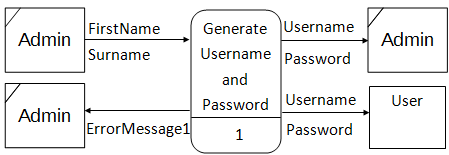
\includegraphics[width=\textwidth]{C:/Users/Jordan/git/COMP4Coursework2/dataflowdiagram1.png}
    \caption{The process of how the administrator puts their classes names into the system} \label{fig:print_function_result}
\end{figure}

\begin{figure}[H]
    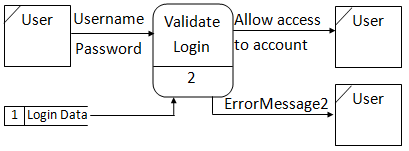
\includegraphics[width=\textwidth]{C:/Users/Jordan/git/COMP4Coursework2/dataflowdiagram2.png}
    \caption{The system validating the users login using the stored login information} \label{fig:print_function_result}
\end{figure}

\begin{figure}[H]
    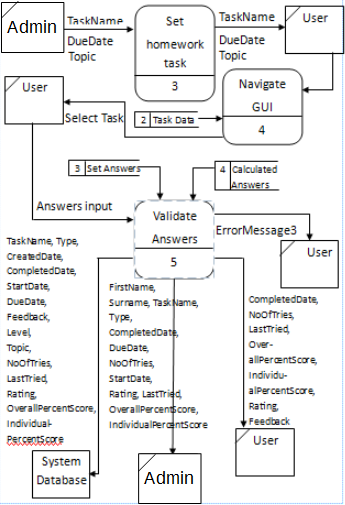
\includegraphics[width=\textwidth]{C:/Users/Jordan/git/COMP4Coursework2/dataflowdiagram3.png}
    \caption{The entire process of a user using the system and the results of a homework being recorded, including the teacher setting the task} \label{fig:print_function_result}
\end{figure}

\subsubsection{Input Forms, Output Forms, Report Formats}

There are no physical forms that are used for input or output; the class names are added into the system manually by the teacher, copying from a register, and output forms always come in the form of an e-mail, or a meeting with parents. Specifically, if a student does not complete homework to a sufficient standard, the teacher manually e-mails the parents personally or calls them in for a meeting. No action is taken by the system beyond informing the teacher of the student's progress.

\textbf{An example register:}

\begin{figure}[H]
    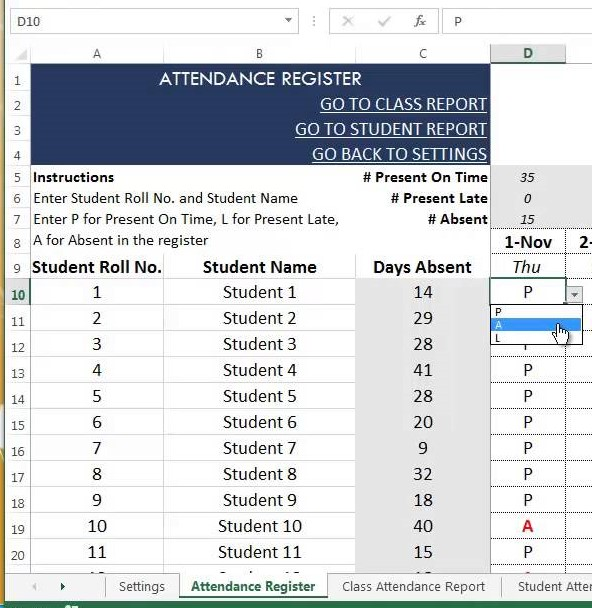
\includegraphics[width=\textwidth]{C:/Users/Jordan/git/COMP4Coursework2/register.png}
    \caption{A screenshot of what the register used to input the names correctly might look like} \label{fig:print_function_result}
\end{figure}

\textbf{An example e-mail to a parent:}

Dear Sir/Madam

I am writing to inform you that your son/daughter has unfortunately not been completing their homework to the standard that is expected of them. 

They have many outstanding tasks to complete, and if they do not complete them very soon I am afraid I will have to call you in for a meeting.

Yours faithfully, \\
Ms Teacher

\subsection{The proposed system}

\subsubsection{Data sources and destinations}

\begin{center}
\begin{tabular}{|p{2.5cm}|p{2.5cm}|p{2.5cm}|p{2.5cm}|p{2.5cm}|}
\hline
\textbf{Source} & \textbf{Data} & \textbf{Process} & \textbf{Example Data} & \textbf{Destination} \\ \hline
Administrator & User ID & The user ID is automatically generated when a class is added to the system & 0001, integer & Database, User \\ \hline
Administrator & Password & The user's password is automatically generated when a UserID is generated & d4g5s1g & Database, User \\ \hline
Administrator & First name & The first name of each user is manually input by the administrator & John, string & Database, User \\ \hline
Administrator & Surname & The surname of each user is manually input by the administrator & Smith, string & Database, User \\ \hline
User & Overall percentage score & The percentage of the questions in a task which the user got correct is recorded automatically upon submission by the system & 70\%, real & Administrator, Database, User \\ \hline
User & Individual question percentage score & The percentage score for each individual question is recorded automatically upon task submission & 50\%, real & Administrator, Database, User \\ \hline
\end{tabular}
\end{center}

\begin{center}
\begin{tabular}{|p{2.5cm}|p{2.5cm}|p{2.5cm}|p{2.5cm}|p{2.5cm}|}
\hline
\textbf{Source} & \textbf{Data} & \textbf{Process} & \textbf{Example Data} & \textbf{Destination} \\ \hline
System & Rating & A red, amber or green face is recorded for each submitted assignment to represent whether or not the user did well enough & Green face graphic, blob & Administrator, Database, User \\ \hline
Administrator & Feedback & The teacher gives feedback to the user manually & Well done, string & Database, User \\ \hline
Administrator & See after class & The administrator can manually set parameters so that the system knows to inform a student if they need to see the teacher after their next lesson e.g Below 50\% & Yes, boolean &  User \\ \hline
Administrator & Time of appointment & The time for a meeting with the user if they need to see the teacher, input manually be the teacher & 11:00AM, time & Administrator, User \\ \hline
\end{tabular}
\end{center}

\subsubsection{Data flow diagram}

\begin{figure}[H]
    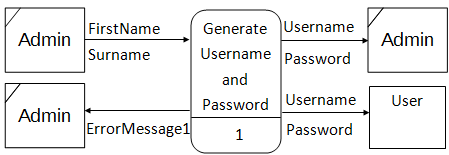
\includegraphics[width=\textwidth]{C:/Users/Jordan/git/COMP4Coursework2/dataflowdiagram1.png}
    \caption{The process of how the administrator puts their classes names into the system} \label{fig:print_function_result}
\end{figure}

\begin{figure}[H]
    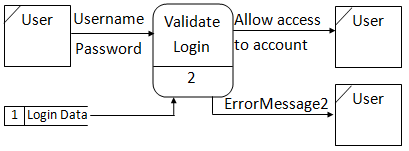
\includegraphics[width=\textwidth]{C:/Users/Jordan/git/COMP4Coursework2/dataflowdiagram2.png}
    \caption{The system validating the users login using the stored login information} \label{fig:print_function_result}
\end{figure}

\begin{figure}[H]
    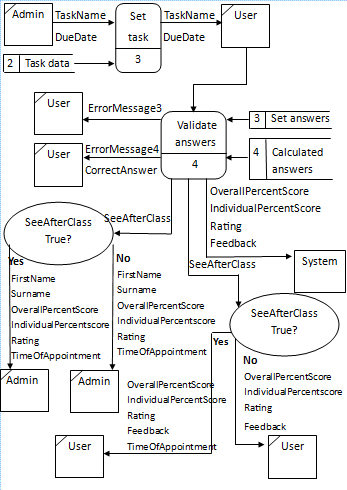
\includegraphics[width=\textwidth]{C:/Users/Jordan/git/COMP4Coursework2/dataflowdiagram4.png}
    \caption{The teacher sets the task, then the student proceeds to complete it, and their progress is recorded} \label{fig:print_function_result}
\end{figure}

\subsubsection{Data dictionary}

\begin{center}
\begin{tabular}{|p{3.4cm}|p{1.2cm}|p{2cm}|p{2cm}|p{2cm}|p{3.5cm}|}
\hline
\textbf{Name} & \textbf{Data Type} & \textbf{Length} & \textbf{Validation} & \textbf{Example Data} & \textbf{Comment} \\ \hline
UserID & Integer & 4 bits & 0001 to 9999 & 1546 & Unique to each user \\ \hline
Password & String and integers & 7 characters & letter followed by number followed by letter & f7h3j5f & The password generator uses mixed data types to avoid inappropriate passwords \\ \hline
FirstName & String & 15 characters & First letter upper case, rest lower case & John & Unique to each user, but could be shared by some \\ \hline
Surname & String & 25 characters & First letter upper case, rest lower case & Smith & Unique to each user, but could be shared by some \\ \hline
TaskName & String & 25 characters & & Trigonometry 2 & Hard-coded into the system \\ \hline
OverallPercentScore & Real & 3 characters & in range 0 - 100 & 76.5\% & The percentage of marks obtained in a test, decimal points allowed \\ \hline
IndividualPercentScore & Real & 3 characters & in range 0 - 100 & 45.5\% & The percentage of marks for an individual question, field will only appear in separate table for individual tasks \\ \hline
Rating & Blob & 64 kilobytes & \ &  Green face graphic & Green, amber or red face graphic \\ \hline
Feedback & String & 500 characters & \ & Good work & This can consist of any characters as it is a personal message \\ \hline
SeeAfterClass & Boolean & 3 characters & Yes or No & Yes & If the user doesn't achieve a sufficient score, this variable will become true and alert the user \\ \hline
AppointmentTime & Time & 5 characters & 24 hour format & 13:35 & Only relevant if the user has a true SeeAfterClass variable, set automatically bsed on the administrator's timetable but can be changed if necessary\\ \hline
\end{tabular}
\end{center}

\begin{center}
\begin{tabular}{|p{3.4cm}|p{1.2cm}|p{2cm}|p{2cm}|p{2cm}|p{3.5cm}|}
\hline
\textbf{Name} & \textbf{Data Type} & \textbf{Length} & \textbf{Validation} & \textbf{Example Data} & \textbf{Comment} \\ \hline
ErrorMessage1 & String & 50 characters & & Sorry, the name cannot have integers & An error message if the wrong data type is used to input a name \\ \hline
ErrorMessage2 & String & 50 characters & & Sorry, that is not a valid login & Tells the user if they have input the wrong username or password \\ \hline
ErrorMessage3 & String & 50 characters & & Please input a decimal, not an integer & Tells the user if their incorrect answer is the wrong data type \\ \hline
ErrorMessage4 & String & 50 characters & & That is incorrect, try one more time & Tells the user that their answer is incorrect and gives them one more attempt \\ \hline
CorrectAnswer & Integer, Real, String & 5 characters & Must be a decimal or whole number, or text if in a text box & 25.5cm & Gives the user the correct answer if they get the question wrong too many times \\ \hline
Login data & String & 25 characters & & johnsmith1, f8j4h6k & The login information saved in the system to be loaded and checked with the user's inputs \\ \hline
Task data & String & 100 characters & & Trigonometry - sin rule, Level 7, Trigonometry & Contains all the information about the task, what difficulty it is, what type it is etc. \\ \hline
Set answers & Integer, Real, String & 5 characters & Must be a decimal or whole number, or text if in a text box & 45{$^o$} & Contains all the set answers for some of the tasks \\ \hline
Calculated answers & Integer, Real & 5 characters & Must be the same as the solution obtained from the algorithm & 29.8 & Contains algorithms which find and validate the solution for randomly generated tasks \\ \hline
\end{tabular}
\end{center}

\subsubsection{Volumetrics}

There are between 25 and 30 students in each class in years 10 and 11, and there are about 10 classes between the two years at the client's school. This equates to 300 students, so 300 records will be needed across the first year. These will not be needed once a year group moves on, so 150 will be overwritten by 150 more, meaning no expansion will be necessary. Obviously there won't be exactly 150 in each year, so there will be a boundary of 30 more or less per year. It is highly unlikely that more would be needed. There will be a total of 360 record spaces each year, half of which will be either overwritten or just deleted following a decline in numbers. Each of these 360 students will have a record with personal details, and then will also have space for 30 more records, easily enough for the amount of tasks they could complete. 360 * 20 is 7600 task records, added to the personal records, making the total number of records in the master database 7960.

Each user's personal record will look like this:

\begin{center}
\begin{tabular}{|p{2.5cm}|p{2.5cm}|p{2.5cm}|p{2.5cm}|p{2.5cm}|} \hline
\textbf{First Name} & \textbf{Surname} & \textbf{UserID} & \text{Password} \\ \hline
John & Smith & john\_smith\_1 & s3g6h3f \\ \hline
\end{tabular}
\end{center}

Each user's task record will look like this:

\begin{center}
\begin{tabular}{|p{4.2cm}|p{2.5cm}|p{3.7cm}|p{4.1cm}|} \hline
\textbf{UserID} & \textbf{TaskName} & \textbf{OverallPercentScore} & \textbf{IndividualPercentScore1} \\ \hline
john\_smith\_1 & Trigonometry Higher & 75\% & 100\% \\ \hline
\textbf{IndividualPercentScore2} & \textbf{Rating} & \textbf{Feedback} \\ \hline
50\% & [Green face] & Very good \\ \hline
\end{tabular}
\end{center}

SeeAfterClass and TimeOfAppointment will not need to be recorded, only the user and the teacher temporarily need to know these.

\section{Objectives}

\subsection{General Objectives}

\subsection{Specific Objectives}

\subsection{Core Objectives}

\subsection{Other Objectives}

\section{ER Diagrams and Descriptions}

\subsection{ER Diagram}

\subsection{Entity Descriptions}

\section{Object Analysis}

\subsection{Object Listing}

\subsection{Relationship diagrams}

\subsection{Class definitions}

\section{Other Abstractions and Graphs}

\section{Constraints}

\subsection{Hardware}

\subsection{Software}

\subsection{Time}

\subsection{User Knowledge}

\subsection{Access restrictions}

\section{Limitations}

\subsection{Areas which will not be included in computerisation}

\subsection{Areas considered for future computerisation}

\section{Solutions}

\subsection{Alternative solutions}

\subsection{Justification of chosen solution}
